\begin{figure}[hbt]
    \centering
    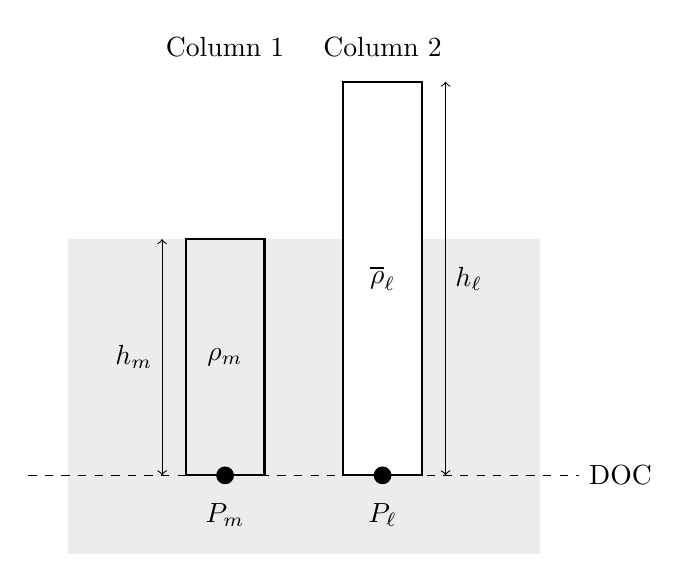
\begin{tikzpicture}[scale=1.0]

        % Asthenosphere
        \fill[gray!15] (-1.5,-1) rectangle (4.5,3);

        % Elevation difference
        \draw[<->] (-0.3,0) -- (-0.3,3) node[midway,left] {$h_m$};

        \draw[thick] (0,0) rectangle (1,3);
        \node[above] at (0.5,5.2) {Column 1};
        \draw[fill=black] (0.5,0) circle (3pt);
        \node at (0.5,1.5) {$\rho_m$};
        \node at (0.5,-0.5) {$P_m$};

        % Columns 1
        \draw[thick,fill=white] (2,0) rectangle (3,5);
        \node[above] at (2.5,5.2) {Column 2};
        \draw[fill=black] (2.5,0) circle (3pt);
        \node at (2.5,-0.5) {$P_\ell$};

        % Heights
        \draw[<->] (3.3,0) -- (3.3,5) node[midway,right] {$h_{\ell}$};

        % Compensation depth
        \draw[dashed] (-2,0) -- (5.0,0) node[right] {DOC};

        % Labels
        \node at (2.5,2.5) {$\overline{\rho}_{\ell}$};

    \end{tikzpicture}
    \caption{Schematic columns for the mantle and a column of lithosphere buoyantly supported at isostatic equilibrium. Pressure is balanced at a depth of compensation (DOC).}
    \label{fig:columns1}
\end{figure}